% Shared preamble for the English summaries in this repository.
\documentclass[11pt,a4paper]{article}
\usepackage[margin=2.2cm]{geometry}
\usepackage[T1]{fontenc}
\usepackage[utf8]{inputenc}
\usepackage{lmodern}
\usepackage{amsmath,amssymb}
\usepackage{graphicx}
\usepackage{booktabs}
\usepackage{enumitem}
\usepackage[hidelinks]{hyperref}
\setlist{itemsep=2pt,topsep=4pt}
\setlength{\parindent}{0pt}
\setlength{\parskip}{5pt}
\graphicspath{{figures/}}
\newcommand{\summaryheader}[3]{%
  \begin{center}
    {\Large\bfseries #2}\\[3pt]
    {\large #1}\\[3pt]
    {\small Arshia Goshtasbi \textbullet{} MSc Electrical Engineering (Control), Iran University of Science and Technology \textbullet{} #3}
  \end{center}
  \vspace{2pt}\hrule\vspace{8pt}
  \noindent\textit{English summary of my original Persian report, which is kept as a PDF in this folder.}\par}

\begin{document}
\summaryheader{Adaptive Control, Homework 7}{Gain Scheduling: Compensating a Nonlinear Valve (Åström \& Wittenmark, Example 9.1)}{Autumn 1404 (2025)}

Both cases are subsystems of \texttt{HW7.slx}. A process is driven through a valve with a nonlinear characteristic. Following the book, I compensated the valve with an approximate inverse of its characteristic, built as a piecewise-linear function with four segments, so that the loop sees a roughly linear actuator. I simulated two versions of the loop and plotted the output against the reference.

\begin{center}
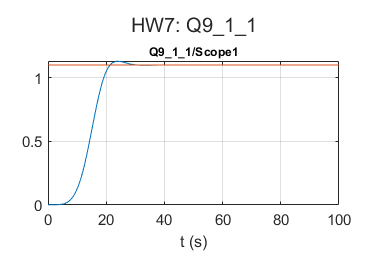
\includegraphics[width=0.45\linewidth]{Q9_1_1.png}\hfill
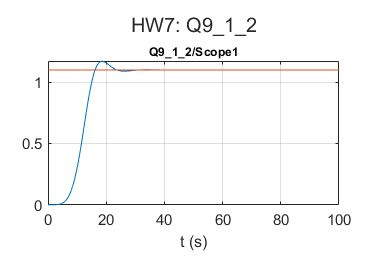
\includegraphics[width=0.45\linewidth]{Q9_1_2.png}\\[2pt]
{\small Re-run in R2023b: the two sub-models of \texttt{HW7.slx}.}
\end{center}
\end{document}
